\documentclass[noinfobox]{mdolab-article}
\usepackage[sort&compress,numbers]{natbib}
\usepackage{enumitem}
\usepackage{booktabs}

% Graphics settings
\graphicspath{{figures/}}
\DeclareGraphicsExtensions{.pdf,.png}

% --- Notation shortcuts -------------------------------------------------
\newcommand{\nstages}{s}                        % number of PCR stages
\newcommand{\Gcoal}{G_{\mathrm{coal}}}          % coalescence gain
\newcommand{\Gocc}{G_{\mathrm{occ}}}            % occupancy gain
\newcommand{\Cpcr}{C_{\mathrm{PCR}}}            % relative cost of one PCR stage
\newcommand{\Tfloor}{T_{\mathrm{floor}}}        % Thomas cost floor
\newcommand{\code}[1]{\texttt{#1}}

% --- Draft note macro (remove once the document is finished) ------------
\newcommand{\todo}[1]{\textcolor{red}{\textbf{[TODO: #1]}}}

\title{A Hybrid PCR/Thomas ADI Solver for ADflow on the GPU}
\author{Safa A. Bakhshi}
\affil{Department of Aerospace Engineering, University of Michigan, Ann Arbor, MI, 48109}
\keywords{ADflow,GPU,CUDA,ADI,tridiagonal solver,parallel cyclic reduction}
\date{\today}

\begin{document}

\maketitle

\begin{abstract}
We implement a GPU native ADI solver in ADflow using the NVIDIA HPC SDK and CUDA Fortran.
The solver uses a hybrid Parallel Cyclic Reduction (PCR) / Thomas algorithm, with the ability to automatically select the switch-over point between PCR and Thomas based on the block dimensions and a set of tunable parameters.
We describe that PCR is needed for both occupancy and memory coalescence, how the switch-over point is chosen, and the integer optimization problem solved during preprocessing to pick the number of PCR stages per block and per sweep direction.
To evaluate the solver we perform a benchmark across several meshes for two different directions concluding that using the hybrid algorithm offers significant speed up to 3.3x over pure Thomas.
The performance results from the benchmark show that PCR is effective at addressing both the memoery coalescence and occupancy limitations of pure Thomas.
\end{abstract}

% \tableofcontents

\section{Overview}

ADI stands for Alternating Direction Implicit and is a type of solver used in ADflow in several places.
In a nutshell, ADI is a line solver that involves sweeping across each block in all three directions ($i$, $j$, and $k$).
Along each line of cells in the given direction we solve a tridiagonal linear system.
These systems are independent of one another, which makes this a great fit for the GPU since all the lines can easily be solved in parallel.

The naive implementation assigns the classic Thomas algorithm~\citep{Thomas1949}, which is inherently serial, to each thread, so that one thread solves one line.
We can do better by addressing two key issues: \emph{occupancy} and \emph{memory coalescence}.
This is where PCR comes in.
Hybrid schemes that begin with a parallel reduction and finish with a serial solve are well established on the GPU.
See \citet{Zhang2010} for the CR/PCR variants that motivated this implementation, and \citet{Kim2011} for a hybrid PCR/Thomas solver that uses a more sophisticated PCR formulation.

\section{Why PCR: Occupancy}

PCR stands for Parallel Cyclic Reduction~\citep{Hockney1981} and is an algorithm for solving tridiagonal linear systems.
Unlike Thomas, PCR is massively parallelizable (hence the name).
By itself, PCR is far more suitable for solving a few very large systems, unlike Thomas, which is better at solving many smaller systems.

This is the concept of \emph{occupancy} on the GPU which is defined as the ratio of the number of warps running to the maximum number of active warps.
Basically, you need to feed Thomas, as he is a hungry boy.
You feed the GPU by giving it more systems to solve at the same time, which is why Thomas is good when you have a large number of smaller systems.
PCR, on the other hand, is fed by giving it larger systems, since PCR works by breaking down a large system into many smaller interleaved systems.
Several threads work on a single large system to break it down, hence the larger system feeds PCR.

There comes a point at which a system has been broken down enough that it is advantageous to switch over to Thomas, because he can now be fed properly.
There are blocks with a sufficient number of systems to satisfy Thomas in all three directions out of the box, so we do not need to run PCR there and can go straight to Thomas.
However, long thin blocks (like in the spanwise direction of a wing) are a problem, and that is where PCR comes into play because it breaks down the systems in those long thin directions so that Thomas can be properly fed with many smaller systems.
That is the occupancy problem PCR addresses, but the sweet spot for the switch has to be identified, since PCR has a cost to run and the benefits to Thomas diminish.

\section{Why PCR: Memory Coalescence}

The second issue PCR improves is memory coalescence.
The basic concept is that you want threads that are next to each other (i.e.\ in a warp together) to access memory that is contiguous (or as close to contiguous as possible) in memory.
In the $j$ and $k$ directions this is fine out of the box (which is counterintuitive for Fortran, but believe me, it is), but the $i$ direction is a problem since it is the fastest index in Fortran.
If this were written in C, then $k$ would be the problematic direction.
The lack of contiguous memory access between adjacent threads causes slow memory access on the $i$ direction sweep, since each thread needs a location in memory that is not contiguous with its neighbors.

Believe it or not, we can use PCR to fix this rather than having to do some kind of expensive array transpose.
What is implemented is a \emph{coalesce on row} feature that activates for ADI kernels only for the $i$ direction sweep:

\begin{itemize}[leftmargin=*]
  \item \textbf{System setup and PCR kernels.}
        Coalesce on row forces contiguous threads to work in parallel along a row (where data is contiguous) rather than along the block face.
        This is only a small part of it.
  \item \textbf{Thomas kernel.}
        This is where the real magic happens.
        Thomas is inherently serial, so by default, with no PCR applied, one thread works on each line with no coalesced memory access and the performance is terrible.
        But PCR breaks the system along the line into smaller ones and leaves them interleaved with each other along the line.
        Now parallelism has been introduced where there was none before, and even better, all the threads are coalesced on the row where memory is contiguous in the $i$ direction.
\end{itemize}

So the more PCR you do, the more coalesced you get, the more parallelism you get, and the better it gets.
The problem, again, is that PCR has a cost and the benefits diminish, so there is a sweet spot.

\section{Benchmark Sweep}
\label{sec:benchmark}

We now have two good uses for PCR, but we need to determine how much PCR to run before switching to Thomas in order to get the best performance.
The starting point was a sweep benchmark:

\begin{enumerate}[leftmargin=*]
  \item Two directions were considered, $i$ and $k$, as $j$ is functionally the same as $k$.
  \item Several meshes were generated for each direction, varying the number of cells on the face, which gives the number of systems, $m$, and the length of the line in the given sweep direction, $n$.
        This gives mesh blocks with different aspect ratios for both the $i$ and $k$ directions, including long-thin ones and short-wide ones.
  \item For each mesh, the number of PCR stages in the direction of interest was swept from $0$ to $5$ in increments of one.
  \item Each case ran ten IRS operations, and the median time to run the ADI sweep in the direction of interest was recorded.
        The median run time of each individual kernel in the ADI solver was also recorded using the \code{nsys} profiling tool.
\end{enumerate}

All ADI kernels use a flat thread block size of 256, and PCR uses a total of $n$ threads per line (a few different choices were tried here, but this does not play a big role).

\begin{figure}[htbp]
  \centering
  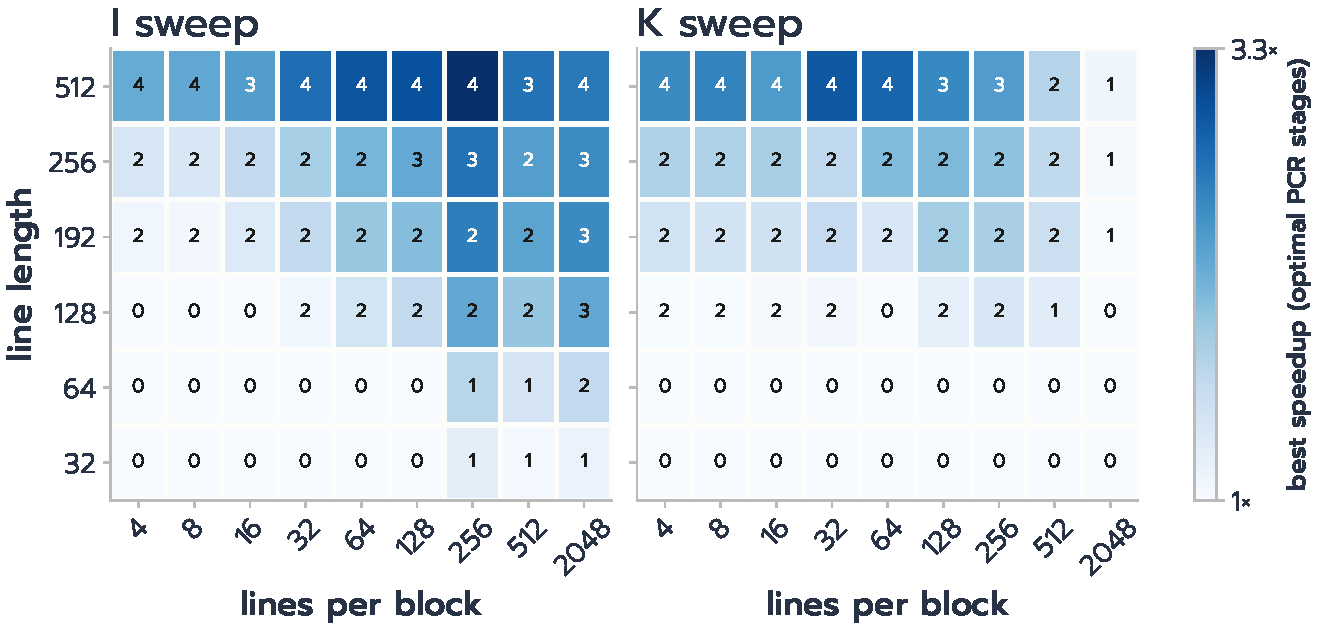
\includegraphics[width=\textwidth]{figures/pcr_speedup_map_v2_new.pdf}
  \caption{Maximum speedup relative to no PCR, and the optimal number of PCR stages that achieves it, for all combinations of $m$ and $n$ in both the $i$ and $k$ directions.}
  \label{fig:sweep}
\end{figure}

For the $k$ direction, where memory coalescence is not an issue, PCR is unsurprisingly advantageous for long thin blocks, as predicted, and in fact gives a decent speedup making implementing PCR already worth it just for dealing with the spanwise direction.
However, the benefit of PCR for introducing memory coalescence in the $i$ direction cannot be understated, as it greatly improves performance for a lot of different block dimensions.

The reason the most speedup is obtained at and beyond 256 lines per block is that the Thomas thread block size is hard-coded to 256 for now.
This is the point at which a single block face occupies a full thread block, which is great for occupancy.
On top of that, PCR chops the line into $2^{\nstages}$ pieces, which means there are $2^{\nstages}$ blocks on a single block face.
Since there is one SM per block, $2^{\nstages}$ SMs work simultaneously, which keeps hungry boy Thomas fed.


\section{Automatic Selection of the Number of PCR Stages}

These parameters can be set manually, but that takes too much time.
Instead, there is a CPU routine that runs during preprocessing and computes the optimal number of PCR stages to use for each block and direction.
We are basically solving a poor man's integer optimization problem here (i.e.\ an \emph{argmin}) subject to two constraints.

\subsection{Objective}

Let $\nstages$ be the number of PCR stages and $n$ the line length in the sweep direction.
The objective is
\begin{equation}
  \label{eq:objective}
  \min_{\nstages}\;
  \Bigl(1 + \nstages\, \Cpcr(\nstages)\Bigr)
  \max\!\left(
    \frac{n}{\max\bigl(\Gcoal,\, \Gocc\bigr)},\;
    \Tfloor
  \right).
\end{equation}

\subsection{Terms}

\begin{description}[leftmargin=*,style=nextline]
  \item[$\Gcoal$ --- coalescence gain]
    The estimated performance gain due to memory coalescence.
    It defaults to $1$ for the $j$ and $k$ directions, and for the $i$ direction is
    \begin{equation}
      \Gcoal = \min\bigl(w,\; 2^{\nstages}\bigr),
    \end{equation}
    where $w$ is the warp size.

  \item[$\Gocc$ --- occupancy gain]
    \begin{equation}
      \Gocc = \min\!\left(
        2^{\nstages},\;
        \max\!\left(\frac{P_{\mathrm{target}}}{n_{\mathrm{lines}}},\, 1\right)
      \right),
    \end{equation}
    where $P_{\mathrm{target}}$ (\code{pcrOccupancyTarget}) can be set by the user or read from the device properties.
    ADflow can now read the device properties and auto-tune based on them.

  \item[$\Tfloor$ --- Thomas cost floor]
    This is the most hand-wavy part.
    It prevents the optimizer from maxing out the PCR stages, since the model otherwise assumes Thomas will just get better and better no matter how many stages are added, which is not the case.
    It is user configurable; $\Tfloor = 44$ was found to be a good default.

  \item[$\Cpcr(\nstages)$ --- cost of one PCR stage relative to Thomas]
    A curve fit, generated from the benchmark data of Section~\ref{sec:benchmark}, that measures the cost of a single PCR stage for a given total number of stages.
    The coefficients of the curve fit are user configurable.
    Figure~\ref{fig:curvefit} documents the curve fit.
\end{description}

\begin{figure}[htbp]
  \centering
  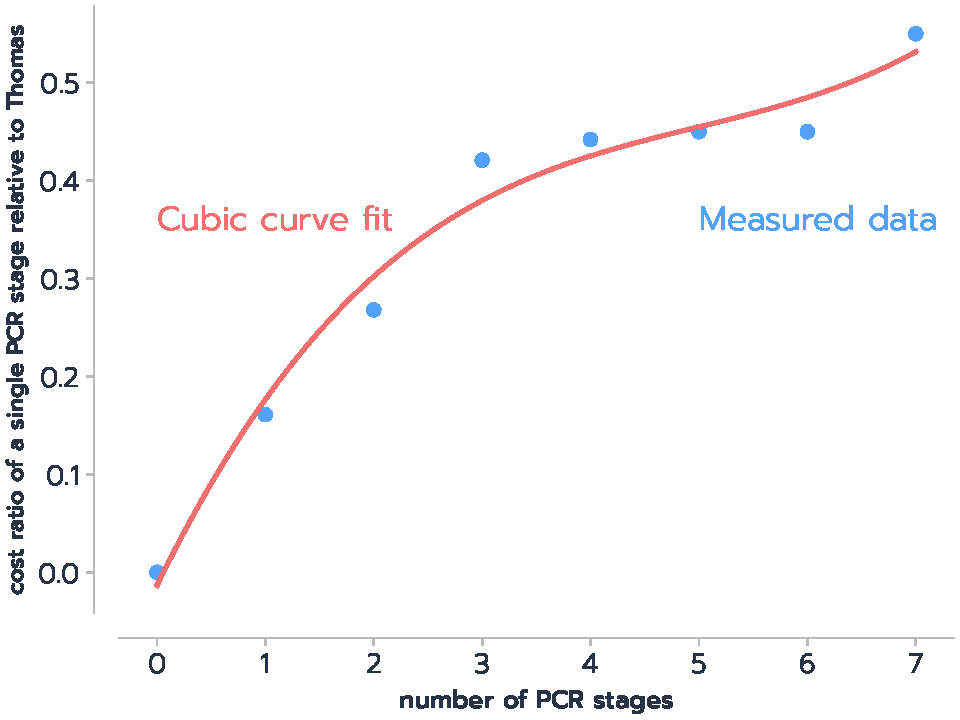
\includegraphics[width=0.5\textwidth]{figures/pcr_cost_model.pdf}
  \caption{Relative cost of a single stage of PCR to Thomas as a function of the total number of PCR stages per ADI sweep.
  The cubic curve fit coefficients are $P_{0} = 0.00269697$, $P_{1} = -0.04027056$, $P_{2} = 0.22761905$, and $P_{3} = -0.01348485$.}
  \label{fig:curvefit}
\end{figure}

\subsection{Constraints}

\begin{enumerate}[leftmargin=*]
  \item \code{minRowsPerPCRThread} sets a floor on the number of rows for a given PCR thread and hence caps the maximum number of PCR threads.
  \item There is a maximum of $\lfloor \log_2 n \rfloor$ PCR stages for a given line length, which cannot be exceeded:
        \begin{equation}
          0 \le \nstages \le \lfloor \log_2 n \rfloor .
        \end{equation}
\end{enumerate}

\section{Where the PCR/Thomas ADI Solver Is Used}

In ADflow we use an ADI solver in three places.

\begin{description}[leftmargin=*,style=nextline]

  \item[Implicit Residual Smoothing (IRS)]
    IRS is only used with the Runge--Kutta (RK) smoother, to implicitly smooth the residuals between stages.
    This effectively replaces the residual in a given cell with a weighted sum of all the residuals in the block, and significantly expands the stability region of the RK smoother so that it allows for much larger CFL numbers, making it more robust.
    For more information on IRS and how it works, see the paper by \citet{Jameson1984}; the multistage RK scheme it accelerates is described by \citet{Jameson1981a}.
    The IRS implementation in ADflow was originally written by Juan Alonso in 2004, and he left a long explanatory comment that is a bit too oversimplified to properly understand what is going on, so I suggest reading the Jameson paper.
    We do not really use the multigrid/explicit RK smoother in ADflow anymore, however this is by far the simplest ADI system in ADflow, making it the best choice to debug and benchmark the ADI solver, so the GPU implementation exists for that reason alone.

  \item[D3ADI Mean Flow Smoother]
    D3ADI stands for Diagonalized Diagonally Dominant Alternating Direction Implicit.
    This is an alternative to the RK smoother in ADflow and, despite the name, is an explicit smoother.
    Generally, it is less robust than RK but can be faster, so in the very rare case where we need the multigrid solver we do use it.
    The scheme combines the diagonalization of \citet{Pulliam1981} with the diagonally dominant factorization of \citet{Bardina1987}, and the combined D3ADI scheme is described by \citet{Klopfer1998}.
    See also the ADflow paper~\citep{Mader2020a} for how the smoother fits into the overall solver.

  \item[Turbulence DADI Smoother]
    Turbulence in ADflow is generally solved in a segregated fashion from the mean flow at all times during an explicit solve and before terminal convergence with NK/ANK.
    A DADI scheme is used \code{nSubiterTurb} times per iteration to resolve the turbulence model for each nonlinear solver iteration.
    Because ANK/NK struggle if the turbulence equation is coupled with the mean flow equation during start-up and intermediate stages of convergence, we still use the turbulence DADI solver in ADflow regularly, and we will need it when the GPU ANK/NK implementations come~\citep{Yildirim2019b}.
    ADflow does couple the turbulence in with the mean flow during terminal convergence (CANK/CSANK iterations) and does have an option to use an implicit step on the segregated turbulence model, but even then we still find the turbulence DADI works the best in many cases.

\end{description}

As explained, the ADI solver will primarily find use in the turbulence DADI routines.
However, having a high performance explicit solver as a solid fallback to ANK/NK on the GPU, where sparse matrix solvers can be a bit underdeveloped, is a valuable capability to have.
Additionally, all three of these ADI solvers in ADflow use an entirely seperate solver implementation so there are actually three ADI solver implementations in ADflow for each of the three applications.
In the GPU implementation, we use a single central implementation with a helper routine to setup the system for each application.


\section{Potential for Further Improvement}

Although we get excellent performance with the PCR/Thomas implementation described here, there is one possible improvement, which involves switching to a tiled PCR algorithm as described by \citet{Kim2011}.
A tiled PCR algorithm divides the system up into tiles and loads them into shared memory with a sliding three-tile window for each given thread.
This enables all the PCR stages to be launched in a single kernel launch, which minimizes the per-stage cost of PCR relative to Thomas.
The number of PCR stages that we currently determine to be optimum in the current PCR/Thomas approach is limited by the cost of PCR relative to Thomas, as captured by $\Cpcr(\nstages)$ in Equation~\eqref{eq:objective}.
If this cost were minimized, we could potentially get one or two more PCR stages for a given sweep.
However, the tiled PCR approach only reduces the cost of PCR, and the potential benefit Thomas can gain from PCR is limited by the floor $\Tfloor$ that we empirically determined.
As a result, we determined that tiled PCR is not worth the implementation effort here.

\bibliographystyle{new-aiaa}
\bibliography{gpu_adi_refs,mdolab}

\end{document}
